\documentclass{article}

\usepackage[top=2cm, bottom=2cm]{geometry}
\usepackage[utf8]{inputenc} % allow utf-8 input
\usepackage[T1]{fontenc}    % use 8-bit T1 fonts
\usepackage{hyperref}       % hyperlinks
\usepackage{url}            % simple URL typesetting
\usepackage{booktabs}       % professional-quality tables
\usepackage{microtype}      % microtypography
\usepackage{graphicx}
%\usepackage{subfigure}
\usepackage{subcaption}
\usepackage{hyperref}       % hyperlinks
\usepackage[dvipsnames]{xcolor}
\usepackage{tikz}           % define for loops


\usepackage{math_commands}

\newtheorem{proposition}{Proposition}
\newcommand*{\expect}[2][]{\ensuremath{\mathbb{E}_{#1} \left[ #2 \right] }} % expectation operator
\newcommand{\logpart}{A}
\newcommand{\conj}{\logpart^*}
\newcommand{\bregman}{\cB_\logpart}
\newcommand{\bregmanconj}{\cB_{\logpart^*}}
\newcommand{\natp}{\theta}
\newcommand{\meanp}{\mu}
\newcommand{\decrement}{D}
\newcommand{\linear}{\ell} % linearization of a function
\newcommand{\lr}{\gamma} % learning rate, or step-size

\newcommand{\MAPm}{\hat \mu_n}
\newcommand{\MAPt}{\hat \natp_n}

\newcommand{\Dir}{\mathrm{Dir}} % Dirichlet
\newcommand{\violet}[1]{\textcolor{violet}{#1}}

\begin{document}

\section{Self-Concordance}

\subsection{Fenchel conjugate motivation to self-concordance}

In the most regular case, when $f(x)$ is a convex function, continuously differentiable on its domain, then its convex conjugate $f^*(y) = \max_x \langle x, y \rangle - f(x)$ verifies
\begin{align}
    \nabla f \circ \nabla f^*  &= \Id \\
     \nabla f^* \circ \nabla f &= \Id
\end{align}
where $\Id$ is the identity function on the relevant domain. In words, the gradients of $f$ and $f^*$ are reciprocal.
Deriving this equality yields
\begin{align}
    \nabla^2 f(x) \nabla^2 f^*(x^*) = I_n
\end{align}
where $x,x^*$ are conjugate points -- e.g. $x^*=\nabla f(x)$ and $x = \nabla f^*(x^*)$.
Now, it gets interesting to us when we derive again this equality. Let's tackle the 1D case first
\begin{align}
    &f''(x) f^{* \prime \prime}(f'(x)) = 1, \forall x \\
    \implies
    &f'''(x)f^{* \prime \prime}(f'(x))  + f''(x)^2 f^{* \prime \prime \prime}(f'(x))  = 0 \\
    \implies
    &\frac{f'''(x)}{f''(x){\frac{3}{2}}}  + \frac{f^{* \prime \prime \prime}(x^*)}{f^{* \prime \prime}(x^*){\frac{3}{2}}}  = 0
\end{align}
where to get to the last line we used the first line, and we divided the second line by $f''(x)^{\frac{1}{2}}$. 
We see that for a pair of conjugate functions, the self-concordance ratio is preserved, modulo the sign.
This gives another rational, beyond dimensional analysis, for using this ratio as a regularity assumption for convex analysis. 

It is also very helpful for us, since we are looking at pairs $\logpart, \conj$, and their associated Bregman divergences. 
If $\logpart$ is SC, then so is 
$f(\natp)= \bregman(\natp ; \natp^*) = \logpart(\natp) - \langle \meanp^*, \natp \rangle + \cst$. 
And $\conj$ is SC as well, thus  $h(\meanp) = \bregmanconj ( \meanp ; \meanp^*)$ is SC.
But there is no reason for 
$g(\meanp) = \bregmanconj ( \meanp^* ; \meanp) =  \cst - \conj(\meanp) - \langle \nabla \conj (\meanp), \meanp^* - \meanp \rangle $ to be SC. 

The multivariate generalization of this formula is a third order tensor equality
\begin{align}
    \nabla^2 f^{-\half} \nabla^3 f \nabla^2 f^{-1} + \nabla^2 f^{* -\half} \nabla^3 f^* \nabla^2 f^{* -1} = 0
\end{align}
where we omit  multiplication axis and functions take relevant argument $x$ or $x^*$. Consequently, a multivariate definition of self-concordance might take the form of an inequality on the 3d tensor $\nabla^2 f^{-\half} \nabla^3 f \nabla^2 f^{-1}$.

\subsection{Suboptimality and Newton Decrement}
An important property of self-concordant functions (cite Boyd's book, although Nesterov's may be better) is that their suboptimality  may be upper bounded by the Newton Decrement 
\begin{align}
    \decrement(x)^2 = \nabla f(x)^T \nabla^2 f(x)^{-1} \nabla f(x) \; .
\end{align}
In general, subtracting the minimum $f^*$ of $f$ , we have
\begin{align}
    f(x) - f* \leq - \decrement(x) - \log( 1- \decrement(x)) \; .
\end{align}
Note that this bound is vacuous for $\decrement(x)\geq 1$. For $y = \decrement(x) \leq 0.68$, we have $ - y - \log(1-y) \leq y^2$, so we get the bound
\begin{align}
    f(x) - f^* \leq \decrement(x)^2 = \nabla f(x)^T \nabla^2 f(x)^{-1} \nabla f(x) \; .
\end{align}

Our functions of interest is $f(\natp)= \bregman (\natp ; \natp^*)= \bregmanconj ( \meanp^* ; \meanp) = g(\meanp)$, with minimum $f^*=0$. 
If $\logpart$ is self-concordant, then so is $f$, but not necessarily $g$.
The gradient and Hessian of $f$ are
\begin{align}
    f(\natp) 
    &= \logpart(\natp) - \logpart(\natp^*) - \langle \meanp^*, \natp - \natp^* \rangle \\
    \nabla f(\natp) 
    &= \meanp - \meanp^* = \expect[p(X|\natp)]{T(X)} - \expect[p(X|\natp^*)]{T(X)} \\
    \nabla^2 f(\natp) 
    &= \mSigma(\natp) = \Cov_{p(X|\natp)}[T(X)]
\end{align}
so that we get the bound.
\begin{align}
    \bregmanconj(\mu^* ; \mu) 
    \leq \decrement(\natp)^2 
    = \norm{\mu^* - \mu(\theta)}^2_{\mSigma(\theta)^{-1}} 
    \leq 0.46
\end{align}
% If we were to use $g(\meanp)$ instead, we would get dirty third order derivatives
% \begin{align}
%     g(\meanp) 
%     &= \conj(\meanp^*) - \conj(\meanp) - \langle \natp, \meanp^* - \meanp \rangle \\
%     \nabla g(\meanp) 
%     &= -\natp - \nabla^2 \conj(\meanp) (\meanp^* - \meanp) + \natp \\
%     &= \nabla^2 \conj(\meanp) (\meanp - \meanp^*) \\
%     \nabla^2 g(\meanp) 
%     &= \nabla^2 \conj(\meanp) + \nabla^3 \conj(\meanp ) (\meanp - \meanp^*)
% \end{align}
% where the last expression involves a third order tensor.

Finally, if instead we were looking at a different function switching the role of $\meanp$ and $\meanp^*$,  $h(\meanp) = \bregmanconj ( \meanp ; \meanp^*)$, then we would get
\begin{align}
    \nabla h(\meanp ) 
    &= \natp - \natp^* \\
    \nabla^2 h(\meanp ) 
    &= \nabla^2 \conj(\meanp) 
    = \nabla^2 \logpart(\natp) ^{-1}
    = \Cov_{p(X|\natp)}[T(X)]^{-1}\\
    \implies 
    \decrement(\meanp)
    &= \Var_{p(X|\natp)}[(\natp - \natp^*)^T T(X)] \; .
\end{align}
This is just a remark. I don't think it can help us to get anywhere. 

\section{MAP on Graphs}
Assume that the variable $X$ factors along some graph $G$. 
We write $G(i)$ the parents of $X_i$ in $G$. 
Then we model the conditional distribution of $X$ given parameter vector $\theta$ factors as
\begin{align}
    p(X|\natp) = \prod_i p(X_i | X_{G(i)};\natp_i)
\end{align}
where $\natp_i$ is the parameter associated to the mechanism $X_{G(i)} \rightarrow X_i$. 
Embracing the Bayesian viewpoint, the independent mechanism principle is embodied as independence between parameters
\begin{align}
    p(\natp) = \prod_i p(\natp_i) \; .
\end{align}
% In other words, we have the following assumptions on $(\natp,X)$
% \begin{align}
%     \indep_{i=1}^d \natp_i \\
%     \natp_i \indep X_{G(i)}
% \end{align}
Following these equations, the joint distribution on $(\natp,X)$ factors along a larger graph $G'$ which augments $G$ by adding nodes $\natp_i$ with arrows pointing to $X_i$, as illustrated in Figure~\ref{fig:joint_graph}.
\begin{figure}[ht]
    \centering
    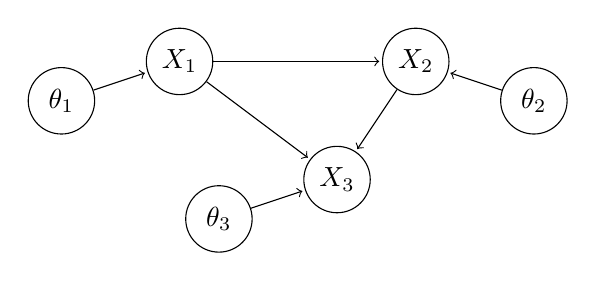
\begin{tikzpicture}[shorten >=1pt,->]
      \tikzstyle{vertex}=[draw, circle,minimum size=24pt,inner sep=0pt]
      \foreach \name/\txt/\x/\y in {x1/X_1/0/0, x2/X_2/3/0, x3/X_3/2/-1.5, t1/\theta_1/-1.5/-0.5, t2/\theta_2/4.5/-0.5, t3/\theta_3/0.5/-2}
        \node[vertex] (G-\name) at (\x,\y) {$\txt$};
    
      \foreach \from/\to in {x1/x2, x2/x3, x1/x3, t1/x1, t2/x2, t3/x3}
        \draw (G-\from) -- (G-\to);
    \end{tikzpicture}
    \caption{A graph $G'$ factorizing $(\natp,X)$. Although the graph restricted on $X$ does not encode any conditional independence, $G'$ does on the joint distribution.}
    \label{fig:joint_graph}
\end{figure}
With such a graph, the Bayesian posterior can be factorized as well
\begin{align}
    p(\natp|X) 
    &\propto  p(X|\natp) p(\natp)& \\
    & = \prod_i p(X_i | X_{G(i)};\natp_i) p(\natp_i)
    &(\indep_i \natp_i) \\
    & = \prod_i p(X_i | X_{G(i)};\natp_i) p(\natp_i\violet{|X_{G(i)}})
    &(\natp_i \indep X_{G(i)}) \\
    & = \prod_i p(X_i, \violet{\natp_i} | X_{G(i)})    &  \\
    & = \prod_i p(\natp_i| \violet{X_i}, X_{G(i)})p(X_i|X_{G(i)})    &  \\
    \implies p(\natp|X) 
    &= \prod_i p(\natp_i| \violet{X_i}, X_{G(i)}) \; .
\end{align}
In words, a consequence of the independence mechanism principle is that the posterior distribution of $\natp_i$ can be inferred solely from $X_i$ and its parents. 

\subsection{Equality of directions for 2 categorical variables}
In my paper on the analysis of causal speed, I proved the equivalence between sampling a joint distribution $\omega = p(A,B) \in \simplex_{K\times K}$ on $(A,B)\in \{1,\dots,K\}^2$ from a Dirichlet with parameter $\gamma\in \real_+^{K\times K}$ and sampling independently the marginal distribution $\mu = p(A)\in \simplex_K$ and the conditional distributions $\nu_i = p(B|A=i)\in\simplex_K$ from Dirichlets with respective parameters $\sum_{j=1}^K \gamma_{:,j} = \gamma \ones$ (matrix vector product) and $\gamma_{i,:}$
\begin{align}
    \underbrace{\Dir_{K^2}((\gamma_{i,j})_{i,j=1}^K) }_{p(\omega)}
    \equiv 
    \underbrace{\Dir_K\left( \gamma \ones \right)}_{p(\mu)} 
    \otimes \left (\bigotimes_{i=1}^K 
    \underbrace{\Dir_K((\gamma_{i,j})_j)}_{p(\nu_i)} 
    \right ) 
    \label{eq:dirichlet_factors}
\end{align}
Seeing data samples $(\cA,\cB) = (A_i,B_i)_{i=1}^n$ as one-hot encodings in $\real^K\times \real^K$, the posterior reads
\begin{align}
p(\mu|\cA) &= \Dir(\gamma\ones + \sum_i A_i)\\
p(\nu_k|\cA,\cB) &= \Dir(\gamma_{k,:} + \sum_i  A_{i,k} B_i ) \\
p(\omega | \cA,\cB) & = \Dir( \gamma + \sum_i A_i B_i^\top )  
\end{align}
where $A_i B_i^\top$ is the one hot matrix encoding of $A,B$.
These three posteriors are obtained independently of each other following rules of calculus for Dirichlet distributions. Yet they happen to define the same distribution on distributions, as we verify below with the two equalities from equation \eqref{eq:dirichlet_factors}.
\begin{align}
    \left(\gamma + \sum_i A_i B_i^\top \right)_{k,l} 
    &= \left(\gamma_{k,:} + \sum_i  A_{i,k} B_i \right)_l \\
    \left(\gamma + \sum_i A_i B_i^\top \right) \ones 
    &= \gamma \ones + \sum_i A_i \; .
\end{align}
The interpretation of this result is that \emph{taking the posterior with the decomposition $A\rightarrow B$ or $B\rightarrow A$ give the same result}. As a corollary the MAP is also the same
\begin{align}
\hat \omega^\text{MAP} 
= \frac{\gamma + \sum_i A_i B_i^\top}{\ones^\top (\gamma + \sum_i A_i B_i^\top) \ones}
=\frac{\gamma + \sum_i A_i B_i^\top}{n_0 + n}
\end{align}
Using Bayesian statistics with this prior, there is no distinction between directions.

Is this bound to happen with a symmetric prior ? Let's give a name to the change of variable $f(\omega) = \mu,\nu$. 
Remark that $f(\omega^\top) = \mu_\leftarrow, \nu_\leftarrow$, eg in the categorical special case transposing omega and changing variables give the anticausal direction. 
For sure  $p(X|\mu,\nu) = p(X|f(\omega)) = p(X|\omega)$. 
Using the change of variable formula  we get something.
But which equality am I looking for exactly ? 
\end{document}